\documentclass[11pt, letterpaper]{article}
\usepackage[margin=0.5in]{geometry}
\usepackage{float}
\usepackage{graphicx}
\usepackage{placeins}

\begin{document}

\title{Boyer Moore vs Naive String Search Comparison}
\author{Jason Hunter}
\maketitle

\section{Introduction}
An organism's DNA contains all the instructions for it's development and function.
It also contains the information that links specific DNA sequences to particular traits or diseases.
In the process of mapping these relationships,
we analyze the DNA of individuals with similar or differing characteristics.
It involves the comparison of sampled DNA sequences to the reference genome.
This can be a computational challenge, as the human genome consists of over 3 billion of these nucleotide base pairs.
Searching through such large sequences requires us to take a look at more efficient algorithms.
The Boyer-Moore algorithm is one such algorithm that can be used to search for a pattern in a text.
It is almost always faster than the naive string search algorithm, which compares the pattern to all possible alignments in the text.
The Boyer-Moore algorithm uses two heuristics, the bad character rule and the good suffix rule, to skip unnecessary comparisons.
Here, I conduct an empirical comparison on the performance of these two algorithms in terms of runtime and memory usage across three experiments: 
a nucleotide base alphabet, an English alphabet, 
and a sequence with repetitive characters representing the worst-case scenario for Boyer-Moore.

\section{Results}
The graphs on the following pages show the runtime and memory usage comparison between the naive and Boyer-Moore search algorithms under different scenarios. 
The x-axis represents the text size, while the y-axis shows the runtime in seconds and memory usage in bytes. The red line represents naive search while the blue line represents Boyer-Moore search.
The pattern size was fixed at 100 characters, and the text size varied from 100 to 10,000 characters in steps of 100.
For each text size, 10 runs were performed to compute average values. The only constant I change
across each experiment is how the text and pattern being compared are generated.

As expected, Boyer-Moore is much faster than the naive search in most cases, especially when the text is composed of several unique characters like the alphabet or nucleotide base pairs.
This is due to Boyer-Moore's ability to skip useless comparisons by use of the bad character table and good suffix rules.
However, in the rare worst-case scenario where the text and pattern are repetitive, Boyer-Moore's performance became even worse than naive search.
In all cases, the memory usage of both algorithms remained relatively constant, with Boyer-Moore using slightly more memory due to the additional heuristic tables it constructs.


%%%%% Add your experiment here %%%%
\center
\subsection{Comparison on Nucleotide Base Alphabet}
\begin{figure}[H]
  \centering
  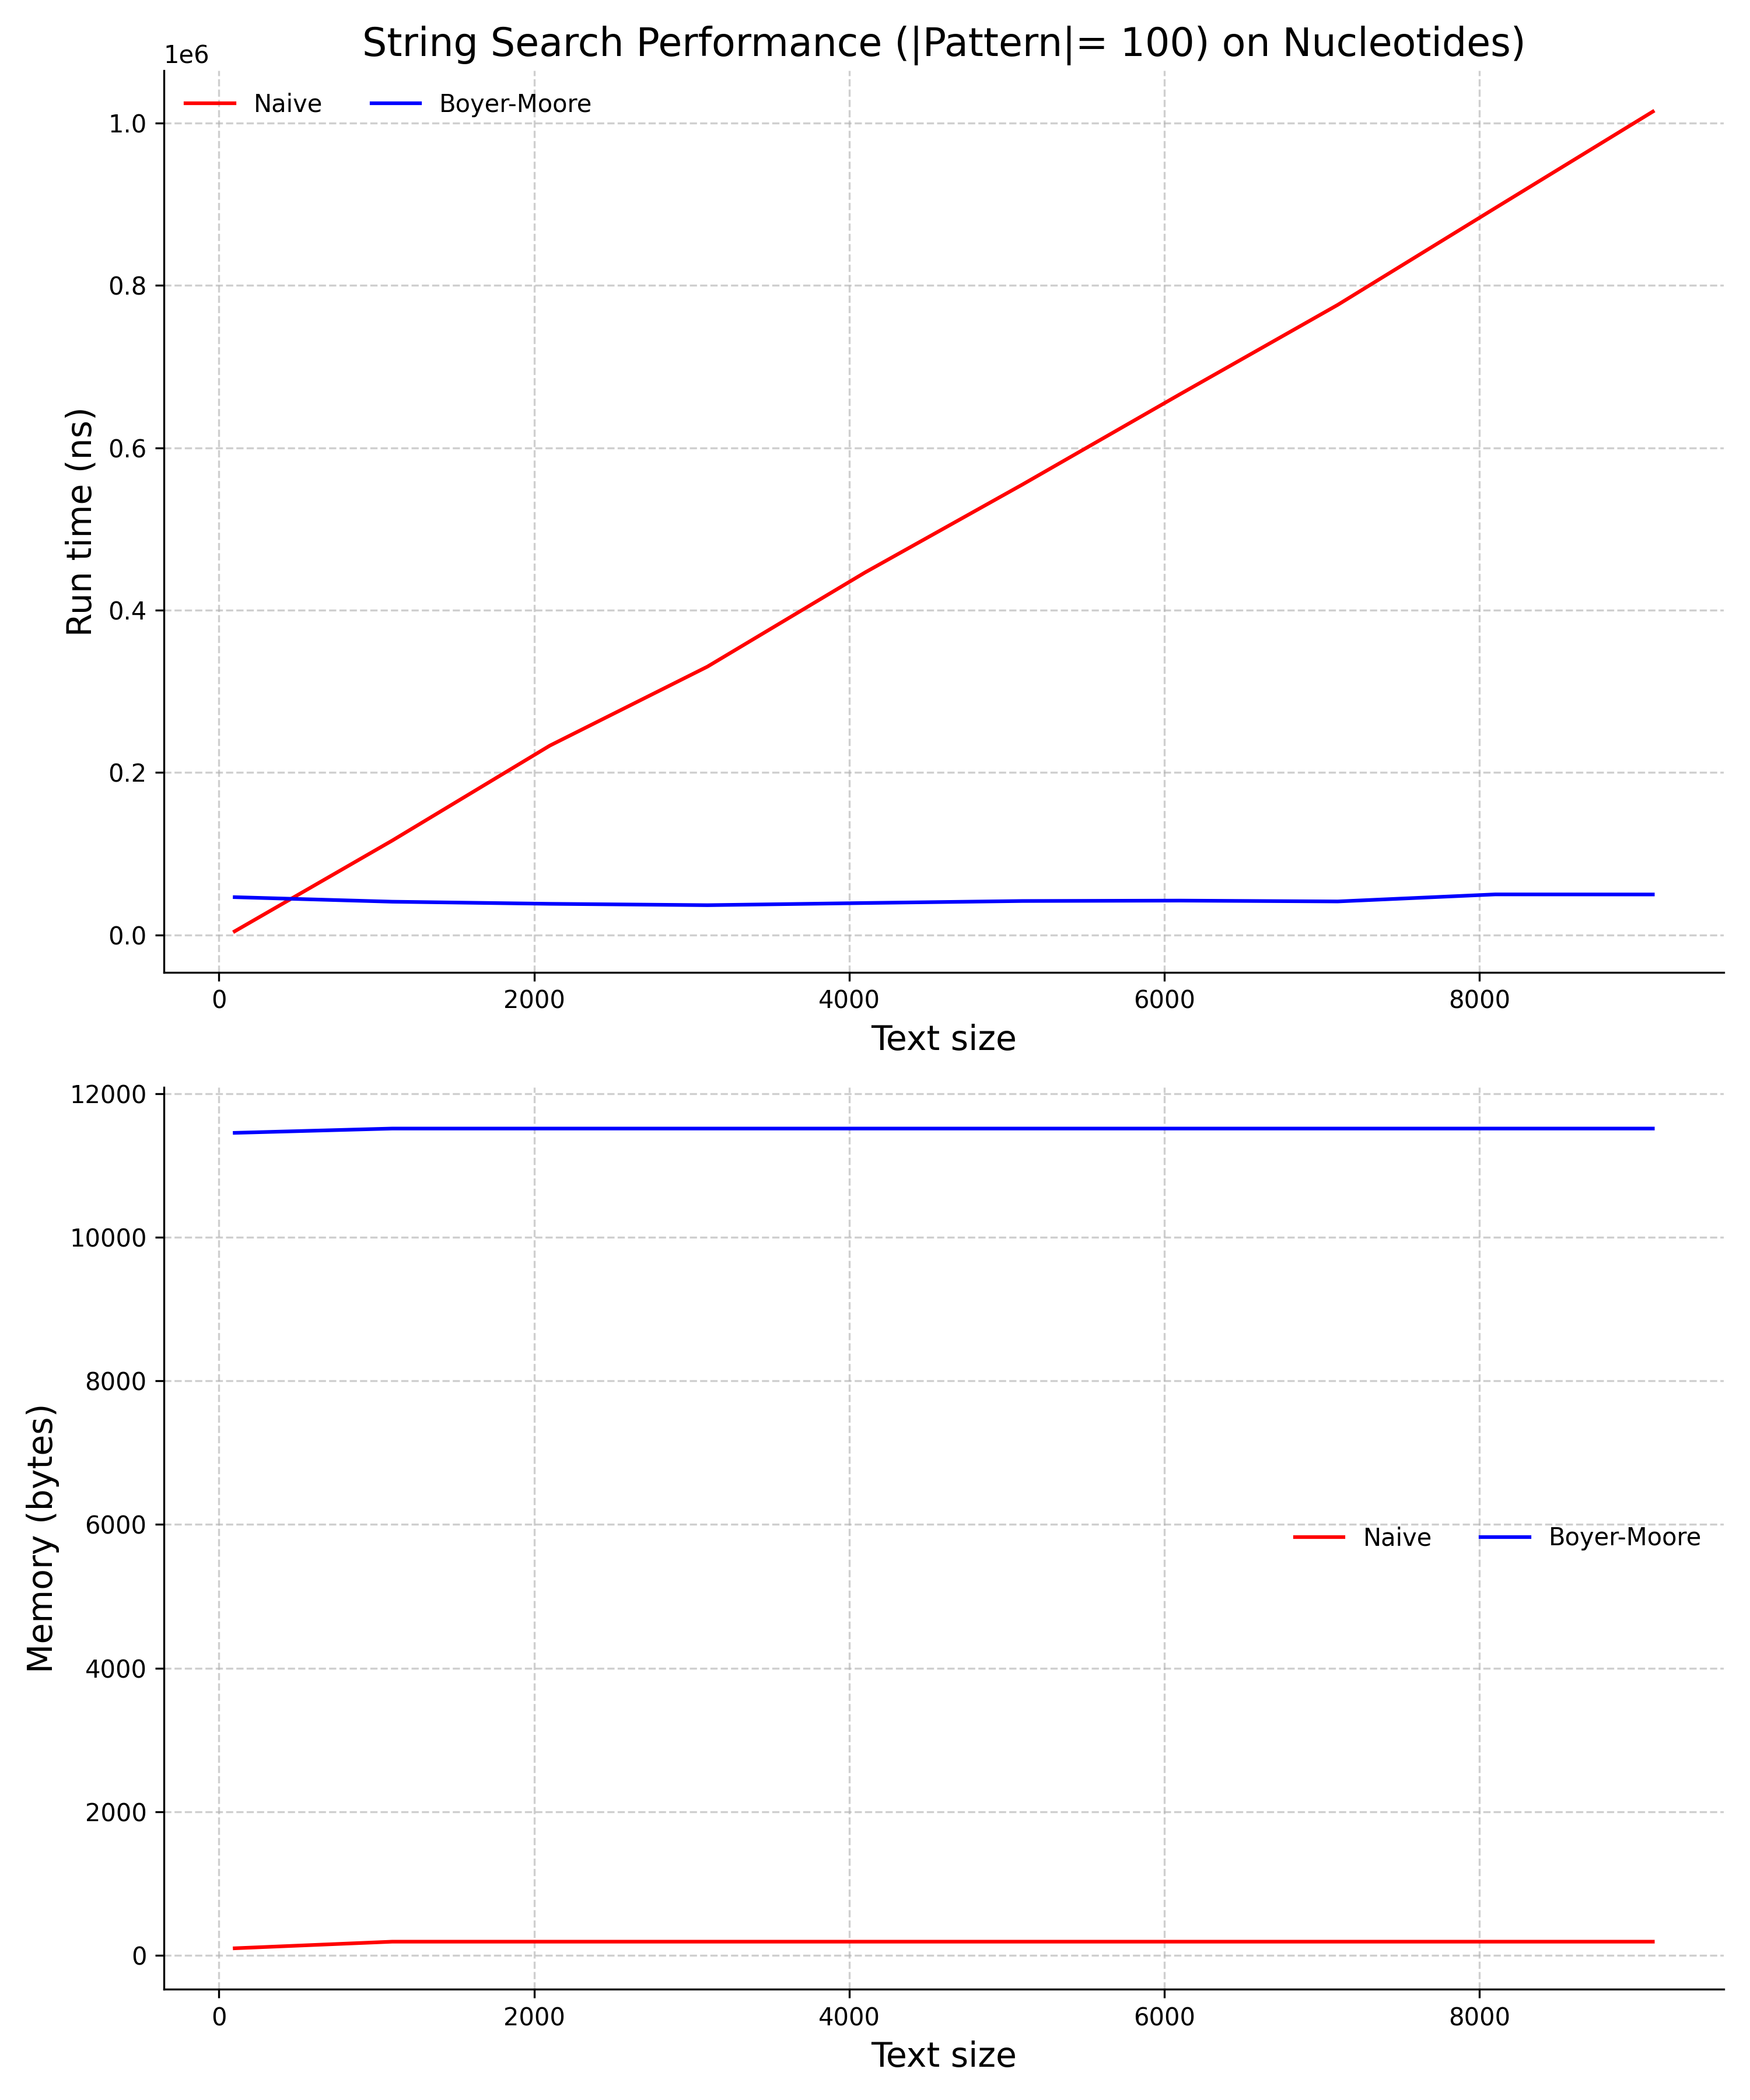
\includegraphics[width=0.8\textwidth]{nucleotide_search.png}
  \caption{Runtime and memory usage comparison between Naive and Boyer-Moore search algorithms using a nucleotide base alphabet.}
  \label{fig:nucleotide}
\end{figure}
\FloatBarrier  % Ensures the figure is placed before proceeding
\flushleft
These are the results obtained when using a nucleotide alphabet. 
The limited alphabet size leads to a higher probability of character matches. 
However, the Boyer-Moore algorithm still outperforms the naive approach in runtime by taking advantage of its heuristic shifts even when mismatches occur.
In experiments using only the four letters representing nucleotides {A, C, T, G}, the limited alphabet size results in a relatively
high chance of character matches. Despite this, the Boyer-Moore algorithm benefits from its heuristic skips when
mismatches do occur, resulting in a significant reduction in runtime compared to the naive approach. This comes at the cost of slightly higher memory usage.

\center
\subsection{Comparison on English Alphabet}
\begin{figure}[H]
  \centering
  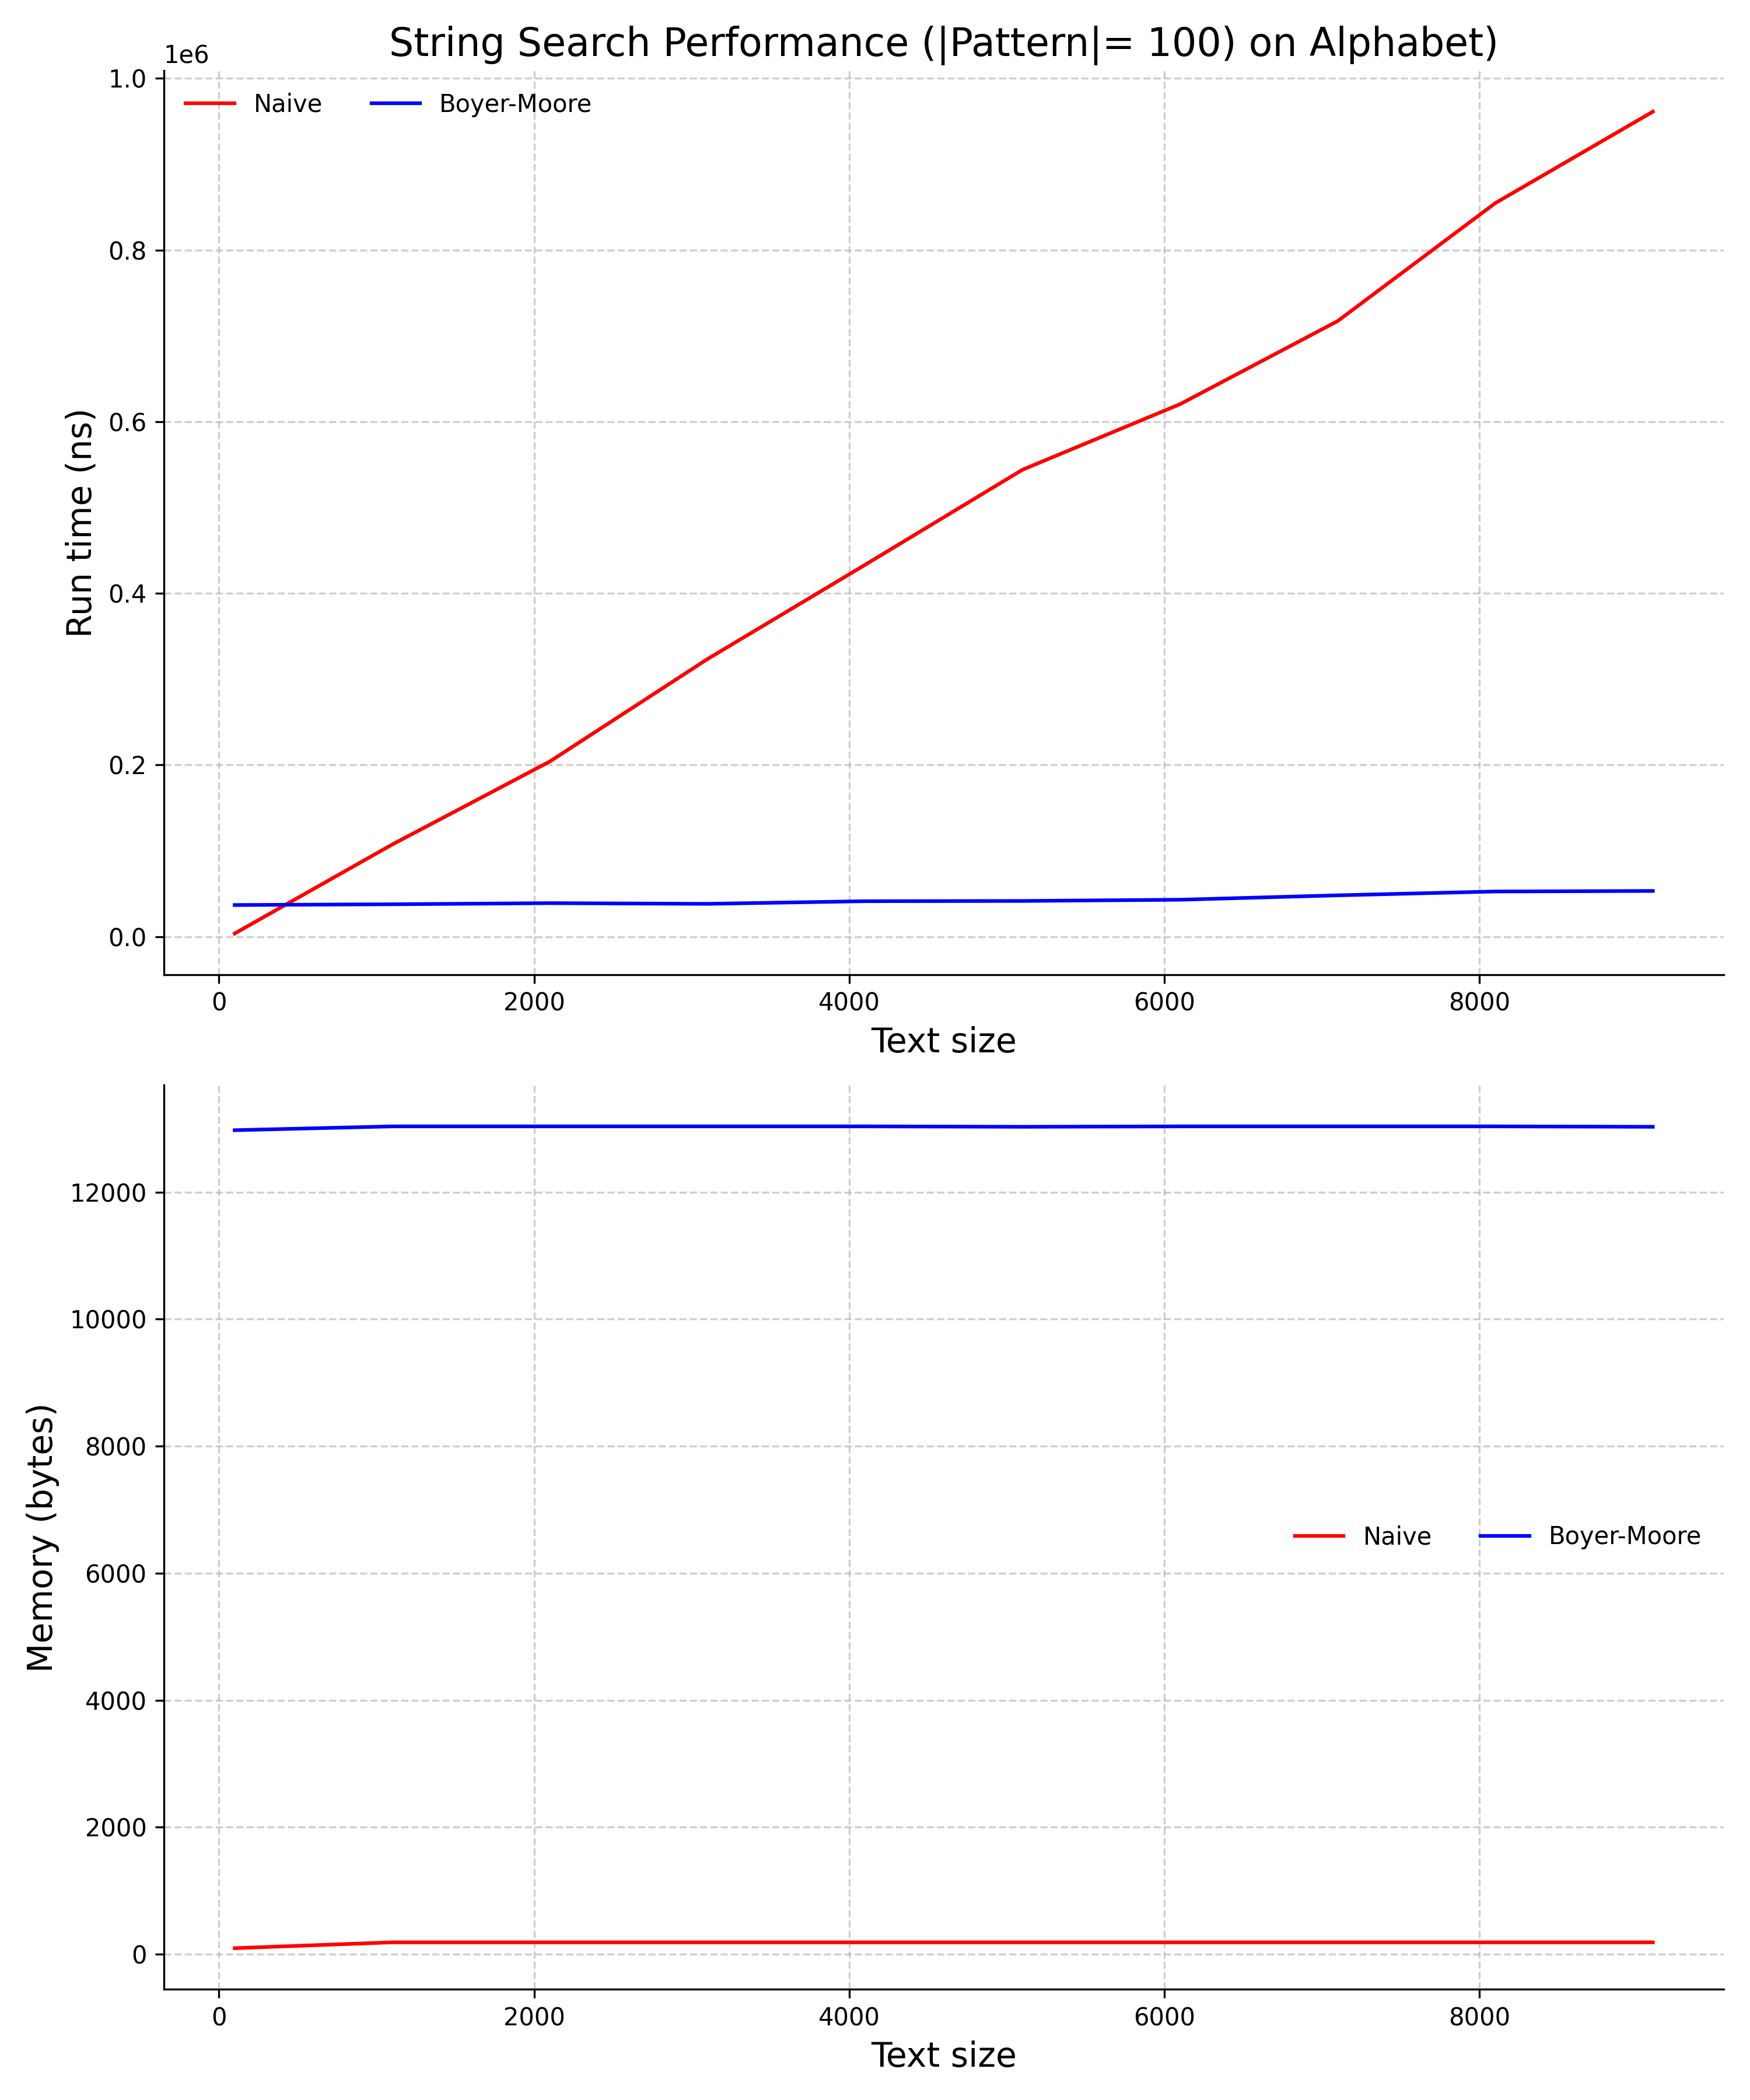
\includegraphics[width=0.8\textwidth]{alphabet_search.png}
  \caption{Runtime and memory usage comparison between Naive and Boyer-Moore search algorithms using the English alphabet.}
  \label{fig:english}
\end{figure}
\FloatBarrier
\flushleft
In this experiment, I added all the characters of the english alphabet to the text and pattern generation process.
With a larger alphabet, the likelihood of a mismatch increases, allowing Boyer-Moore to take advantage of larger shifts.
the probability of encountering a mismatch increases due to the larger alphabet size. 
This higher likelihood of mismatches allows the Boyer-Moore algorithm to take advantage of larger shifts more frequently than in the nucleotide base scenario. 
I expected to see a more pronounced difference in runtime between this and the nucleotide base scenario, but they were quite similar.
The memory use in both cases is uninteresting as it remains constant for both algorithms, citing the same reasons as before.

\center
\subsection{Comparison in Worst-Case Scenario}
\begin{figure}[H]
  \centering
  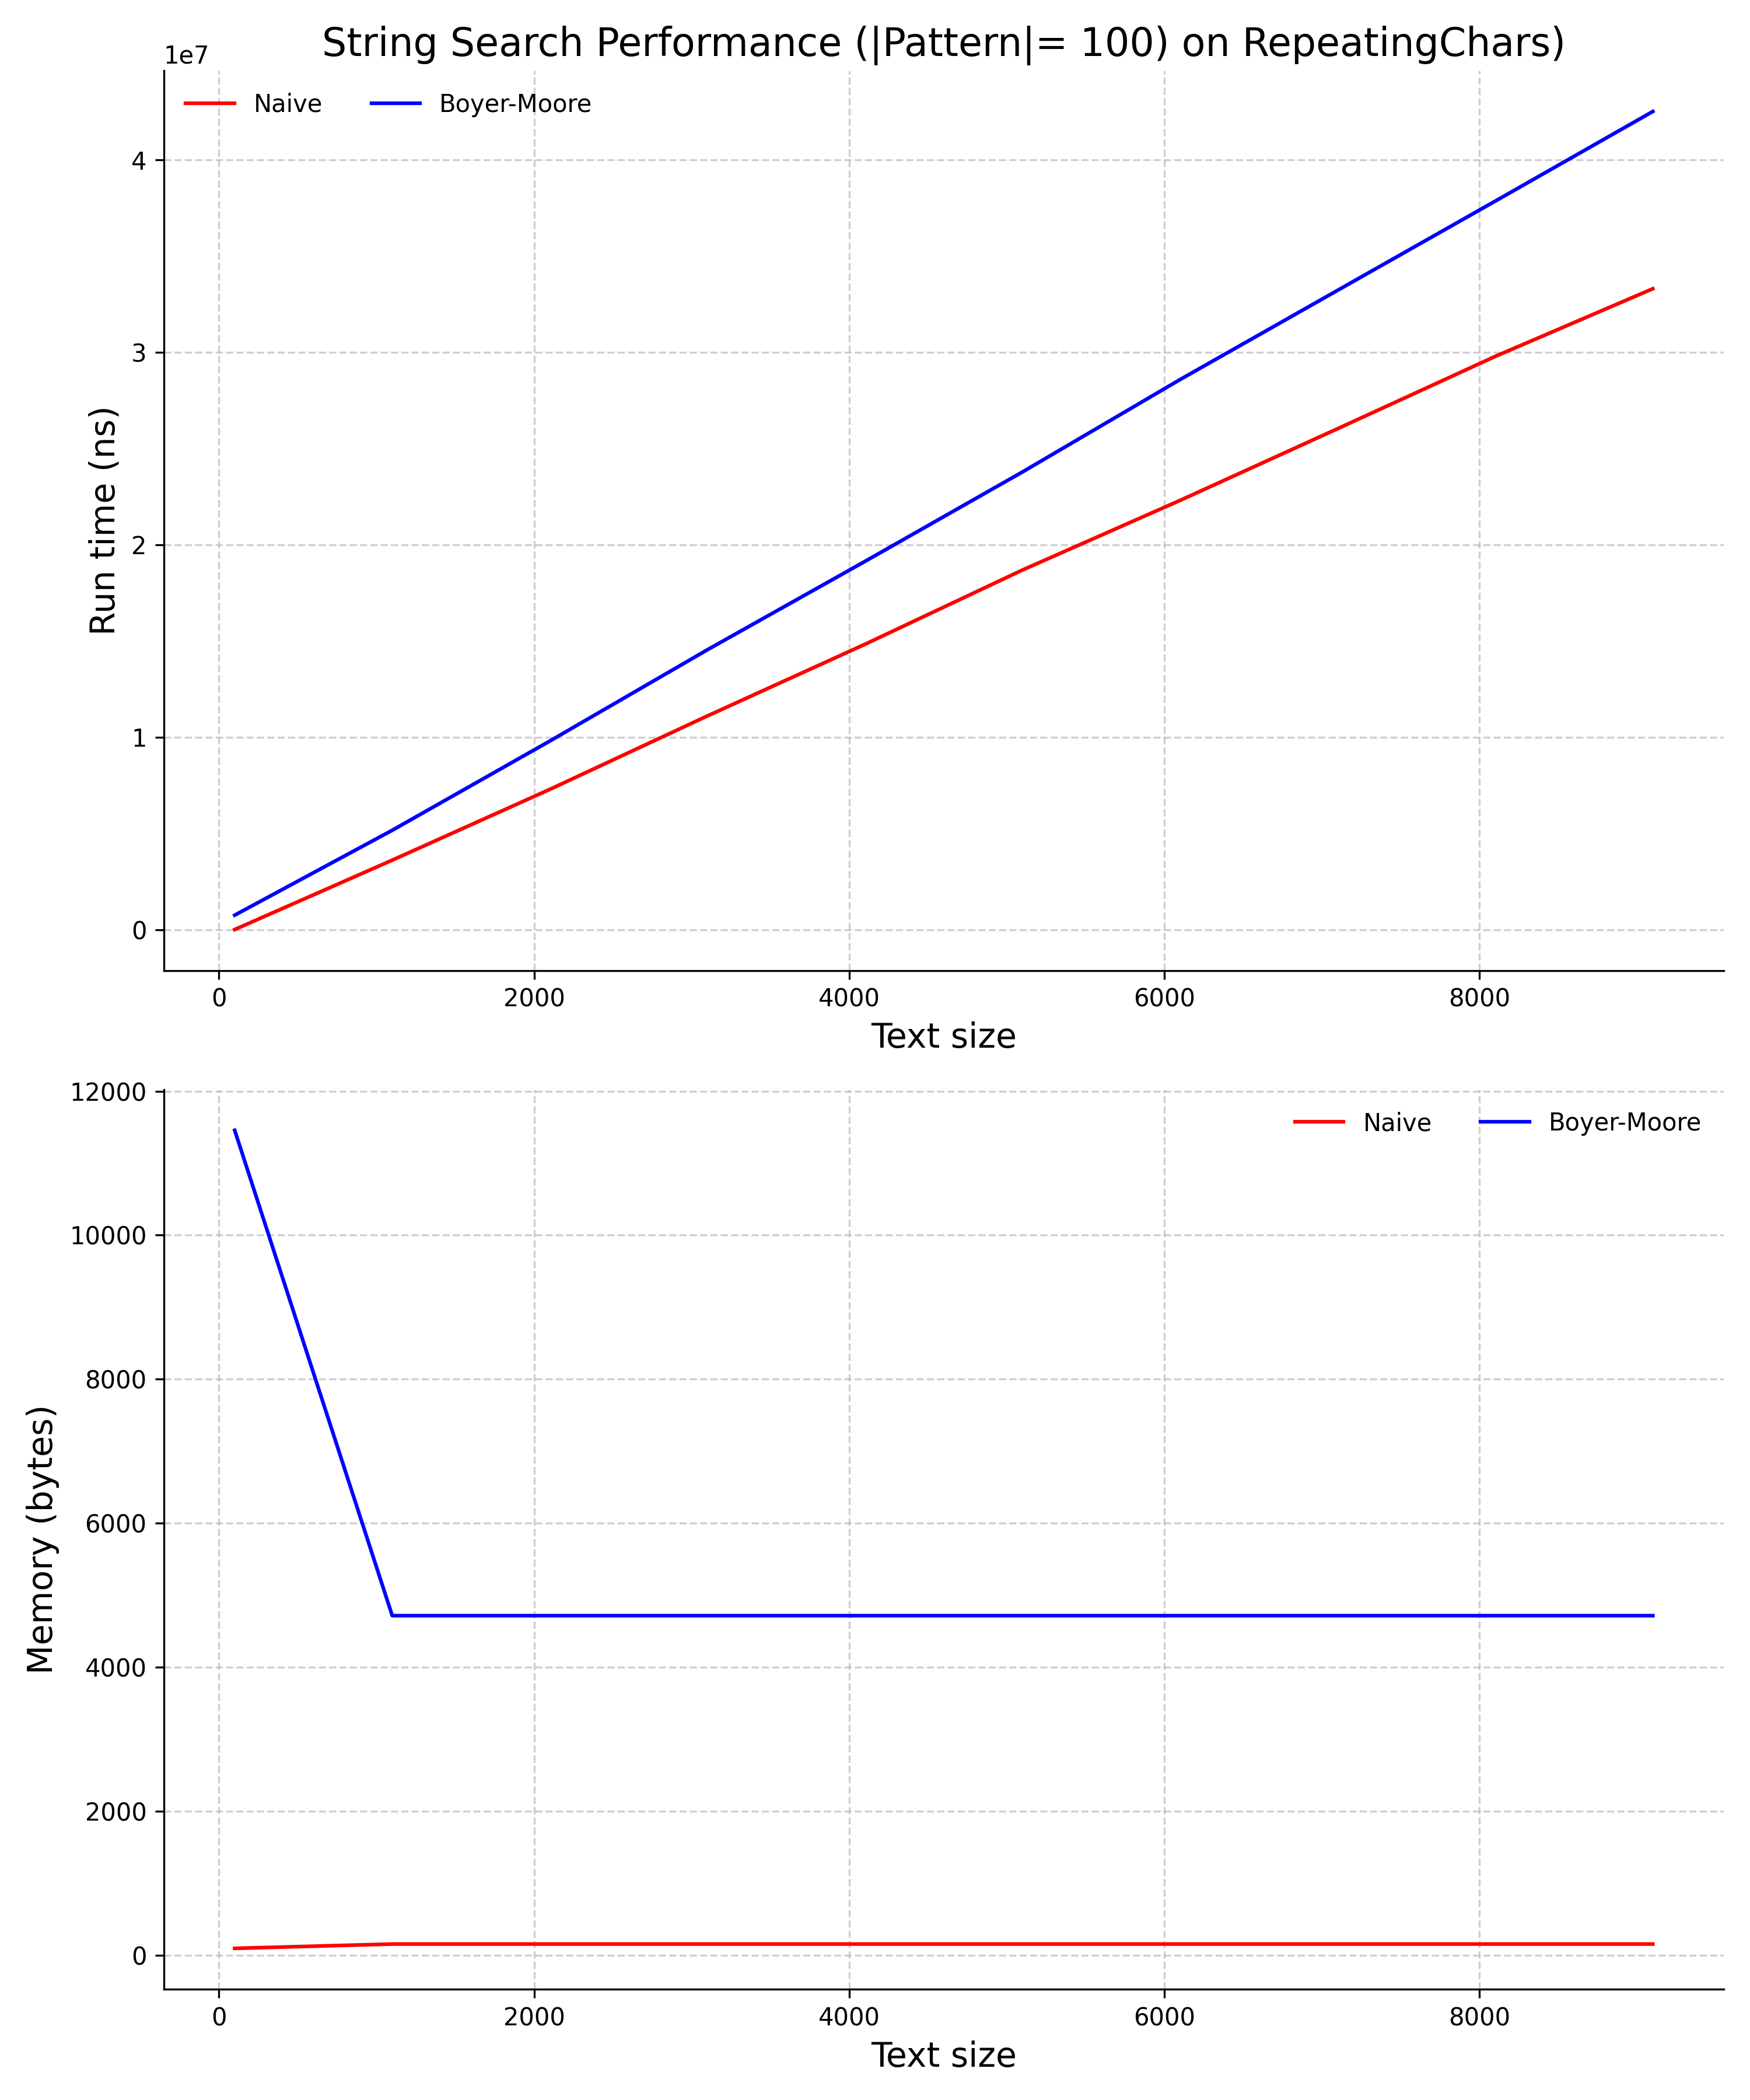
\includegraphics[width=0.8\textwidth]{worstcase_search.png}
  \caption{Performance comparison in the worst-case scenario for the Boyer-Moore algorithm.}
  \label{fig:worstcase}
\end{figure}
\FloatBarrier
\flushleft
In order to simulate the worst-case for Boyer-Moore, I generated both the text and pattern as repetitive strings of the same character.
Under these conditions, the heuristic tables provide minimal benefit and the algorithm's performance essentially becomes that of naive search. 
The worst-case scenario for Boyer-Moore occurs when the text $T$ and the pattern $P$ consist of highly repetitive characters (e.g., $T = \mathtt{AAAA\ldots A}$ and $P = \mathtt{AAAA\ldots A}$).
In this situation, the heuristic tables provide little to no advantage, as mismatches are rare and the potential shifts are minimal. 
Under such conditions, the performance of Boyer-Moore seems to reduce in efficiency to be comparable to, or even slightly worse than the naive string search. 
However, in terms of DNA sequence analysis, the worst-case scenario is highly unlikely to occur in practice, as DNA sequences are almost always composed of non-repetitive nucleotides.

\section{Methods}

\subsection{Naive String Search}
The naive string search algorithm considers all possible alignments of the pattern $P$ with the text $T$.
Starting at the first position in $T$, the algorithm compares $P$'s characters with the corresponding characters in $T$.
If all characters match, the algorithm records the alignment's position in $T$. 
The algorithm then repeats this process for the next alignment. 
If any of the characters in $P$ do not match a corresponding character in $T$, the current alignment is discarded and $P$ shifts one position to the right in $T$,
with the process repeating until all possible alignments have been checked. 
The algorithm then returns the positions at which $P$ was found in $T$.

\subsection{Boyer-Moore String Search}
The Boyer-Moore string search algorithm is an efficient alternative to the naive approach.
This optimization is achieved by preprocessing the pattern $P$ to construct two heuristic tables: the \emph{bad character} table and the \emph{good suffix} table.
These tables are then used to determine how far the pattern can be shifted in the text $T$ when a mismatch occurs.
The algorithm starts by aligning the pattern $P$ with the beginning of the text $T$.
It compares $P$ from right to left with the corresponding characters in $T$.
If a mismatch is found, the algorithm uses the bad character and good suffix tables to determine the largest possible shift that can be made without missing any potential matches.
The bad character table tells how far to shift the pattern based on the mismatched character in $T$, while the good suffix table tells how far to shift based on the matched suffix in $P$.
The largest shift is always chosen to maximize efficiency.
This process repeats until the pattern has been aligned with all possible positions in the text.

\subsection{Empirical Comparison}
I evaluated the performance of both the naive string search and the Boyer-Moore algorithm. 
In the experiments, the pattern size was fixed at 100 characters, 
while the text size varied from 100 to 10,000 characters in steps of 100. 
For each text size, a random text $T$ was generated and a substring $P$ was extracted from it. 
Based on the experiment requested, the alphabet that $T$ and $P$ were drawn from varied.
The performance metrics considered were runtime and memory usage, and for each text size, 
10 runs were performed to compute average values.

\subsection{Reproducibility}
To replicate these experiments, clone the repository and then run the
following commands from the root directory of the repository.
\begin{verbatim}
$ git clone https://github.com/cu-compg-spring-2025/assignment-4-string-search-JasonHunter95.git
$ cd assignment-4-string-search-JasonHunter95
$ python3 src/string_search.py \
--experiment_type Nucleotides \
--text_range 100 10000 1000 \
--pattern_size 100 \
--out_file doc/nucleotide_search.png
\end{verbatim}

\begin{verbatim}
$ python3 src/string_search.py \
--experiment_type Alphabet \
--text_range 100 10000 1000 \
--pattern_size 100 \
--out_file doc/alphabet_search.png
\end{verbatim}

\begin{verbatim}
$ python3 src/string_search.py \
--experiment_type RepeatingChars \
--text_range 100 10000 1000 \
--pattern_size 100 \
--out_file doc/worstcase_search.png
\end{verbatim}

%%%% Add your command here%%%%

\end{document}
